% References:
%
% PMG weak boson wiki
% https://twiki.cern.ch/twiki/bin/view/AtlasProtected/PmgWeakBosonProcesses#Normalisation_discrepancies_due
%
% Differential cross-sections for Z + b-jets at 13 TeV
% https://link.springer.com/content/pdf/10.1007/JHEP07(2020)044.pdf

The production of \PZ bosons in association with jets is estimated
using events simulated with \SHERPA[2.2.1]~\cite{Bothmann:2019yzt}
interfaced to the matrix element generators
\OPENLOOPS~\cite{Buccioni:2019sur,Cascioli:2011va,Denner:2016kdg} and
Comix~\cite{Gleisberg:2008fv} (cf.\ \Cref{tab:monte_carlo} in
\Cref{sec:data_and_simulation}). This generator configuration merges
hard-scatter matrix elements at NLO for final states with up to two
partons with matrix elements at LO for up to four partons. Prior to
the fit, inclusive \Zjets cross sections at
NNLO~\cite{Anastasiou:2003ds} are used for the normalisation of the
background prediction.

% Why IS HF difficult?
% Theory context here: https://arxiv.org/pdf/2204.12355.pdf
The requirement of having two \btagged jets in the signal regions
leads to an enhancement of \PZ bosons produced in association with
quarks of heavy flavour. The modelling of the \ZHF background is
difficult due to its sensitivity to the flavour structure of the
proton and to gluons splitting to bottom or charm
quarks~\cite{Maltoni:2012pa,Napoletano:2018euk,Napoletano:2019tla}. The
nominal prediction of the \ZHF background with \SHERPA, which employs
a five flavour number scheme\footnote{TODO: Explain} for the treatment
of $b$-quarks in the proton, is known to underestimate the \ZHF
contribution~\cite{STDM-2017-38}.
% by \SIrange{10}{30}{\percent} depending on the selected phase
% space~\cite{STDM-2017-38}.
Therefore, the normalisation of the \ZHF background is measured in a
dedicated control region.

% Instead of relying on the normalisation predicted by simulation, the
% normalisation of the \ZHF background is measured in a dedicated
% control region targeting $Z + bb$ production which is then
% extrapolated to the signal regions.

The approach of estimating the \ZHF background described in the
following is adopted with few modifications~\cite{bokan} from the
previous publication in this channel~\cite{HIGG-2016-16-witherratum}
which built on findings from searches of $VH$ ($\PHiggs \to \bbbar$)
production~\cite{HIGG-2016-29}.

% Control region definition
A dedicated control region is defined targeting the production of
$\PZ \ra \Plp\Plm$ ($\ell = e , \mu$) in association with
$b$-jets. The definitions of selected objects used in the control
region and requirements on event quality criteria remain the same as
previously described
in~\Cref{sec:object_reconstruction,sec:event_selection} for
consistency with the signal region selection. Events with same flavour
lepton pairs are recorded using single- and di-lepton
triggers. Thresholds are applied to the \pT of electrons and muons
after offline reconstruction to ensure that the triggers operate close
to their trigger efficiency plateau. Depending on the run conditions
of the LHC, the \pT-thresholds range from \SIrange{25}{27}{\GeV} for
single-electron and \SIrange{21}{28}{\GeV} for single-muon
triggers. Events selected by di-electron triggers need to pass
symmetric \pT-thresholds on both the leading and sub-leading electron
ranging from \SIrange{13}{25}{\GeV}. Events selected by di-muon
triggers are required to pass asymmetric thresholds of
\SIrange{19}{24}{\GeV} on the leading and \SI{10}{\GeV} on the
sub-leading muon. All events are required to be consistent with the
decay of a \PZ boson into electrons or muons in association with
$b$-jets. Leptons are required to be of same flavour with opposite
electric charges and a di-lepton invariant mass between \SI{75}{\GeV}
and \SI{110}{\GeV}. Exactly two \btagged jets are required with the
invariant mass between both jets
fulfilling~$\mBB \not\in [\SI{40}{\GeV}, \SI{210}{\GeV}]$. This
requirement on \mBB had to be introduced to ensure orthogonality with
signal regions of searches for Higgs boson pair production in final
states with $\bbbar\Plp\Plm + \pTmissAbs$.\footnote{For future
  iterations of this search it would be justifiable, based on
  arguments of the larger SM \HH sensitivity of the
  $\bbbar\tau^{+}\tau^{-}$ channel, to forgo the orthogonality
  requirement thus allowing the use a \ZHF control region selection
  more similar to the selections applied for the signal regions of the
  $\bbbar\tau^{+}\tau^{-}$ channel.} After the \ZHF control region
selection, the electron and muon channels are combined for further
analysis.

% Labeling and fit
% https://twiki.cern.ch/twiki/bin/view/AtlasProtected/FlavourTaggingLabeling
Simulated \Zjets events entering the \ZHF control region are
categorised according to a generator-level flavour label assigned to
the pair of $b$-jet candidates. Reconstructed jets are labelled as
either $b$, $c$, or \emph{light} ($l$) according to the presence of
hadrons within a cone of $\Delta R < 0.3$ around the jet axis. If a
$b$- or $c$-flavoured hadron with a transverse momentum of at least
\SI{5}{\GeV} is found within the cone, the jet is labelled $b$ or $c$,
respectively. When a hadron matches multiple jets the ambiguity is
resolved by giving precedence to the closest jet in $\Delta R$. Jets
that are not matched to any $b$- or $c$-flavoured hadrons are labelled
as \emph{light}. Six categories are defined based on the flavour label
of the $b$-jet candidate pair:~$Z + bb$, $Z + bc$, $Z + cc$, $Z + bl$,
$Z + cl$, and $Z + ll$. Contributions from $Z + bb$, $Z + bc$, and
$Z + cc$ are combined and collectively referred to as \ZHF. The
remaining \Zjets events with at least one \emph{light}-jet are
combined into a sample referred to as \ZLF.

% \Zjets events from simulation are partitioned according to the
% flavour labels of the $b$-jet candidates into six categories:
% $Z + bb$, $Z + bc$, $Z + cc$, $Z + bl$, $Z + cl$, and $Z +
% ll$. Contributions from $Z + bb$, $Z + bc$, and $Z + cc$, where both
% $b$-jet candidates are matched to hadrons of heavy flavour at
% generator-level, are combined and collectively referred to as
% \ZHF. The remaining \Zjets events with at least one \emph{light}-jet
% are combined into a sample referred to as \ZLF.

The pre-fit event yield in the \ZHF control region is given
in~\Cref{tab:zcr_yields}. The majority of events in the control region
originate from \ZHF\footnote{About \SI{90}{\percent} of events in the
  inclusive \ZHF sample are $Z + bb$ events.} or top quark pair
production.
% Only about
% 3% of top quark is single top The production of $Z + bb$ accounts for \SI{90}{\percent} of events in the inclusive \ZHF sample.
To distinguish between the \ZHF and \ttbar contributions in the
likelihood fit, the invariant di-lepton mass, \mll, is used as a
discriminant. The \mll distribution prior to the fit is depicted
in~\Cref{fig:zcr_mll_prefit} showing the expected discrepancy between
data and the pre-fit prediction.

\begin{table}[htbp]
  \centering

  \caption{Event yields in the \ZHF control region before (pre-fit)
    and after (post-fit) the binned maximum likelihood fit of the \mll
    distribution in the control region. The \emph{Other} category
    summarises smaller backgrounds and largely consists of events from
    di-boson processes. The uncertainties on the event yield include
    all experimental and systematic uncertainties.}%
  \label{tab:zcr_yields}

  % Pre-fit:
% Other contains:
% ttH & 32.6 $\pm$ 2.8\\
% VBFHtautau & 0.041 $\pm$ 0.041\\
% diboson & 412 $\pm$ 91\\
% W & 21.9 $\pm$ 3.4\\
% DY & 74.8 $\pm$ 5.7\\
% DYtt & 0.052 $\pm$ 0.011\\

% Post-fit of CR only
%
% Other:
% ttH & 32.5 $\pm$ 2.8\\
% VBFHtautau & 0.04 $\pm$ 0.04\\
% DY & 72.6 $\pm$ 5.2\\
% diboson & 402 $\pm$ 88\\
% W & 21.2 $\pm$ 3.2\\
% DYtt & 0.0485 $\pm$ 0.0091\\

\begin{tabular}{l@{\hskip 20pt}S[table-format=5.0(4)]@{\hskip 20pt}S[table-format=5.0(4)]}
  \toprule
  & \multicolumn{2}{c}{Event yield} \\
  \cmidrule{2-3}
  Process & {Pre-fit} & {Post-fit} \\
  \midrule
  $Z \to \ell^+\ell^- + \text{HF}$ & 41200 \pm 3200 & 55700 \pm 1300 \\
  Top-quark & 36600 \pm 1400 & 35260 \pm 370 \\
  $Z \to \ell^+\ell^- + \text{LF}$ & 5300 \pm 1800 &  4500 \pm 1300 \\
  Other & 541 \pm 94 & 528 \pm 90 \\
  \midrule
  Total prediction & 83600 \pm 5200 & 96030 \pm 320 \\
  \midrule
  Observed data & \multicolumn{2}{c}{\num{96032}} \\
  \bottomrule
\end{tabular}


%%% Local Variables:
%%% mode: latex
%%% TeX-master: "../phd_thesis"
%%% End:

\end{table}

% Since the normalisations of \ttbar and \ZHF are extracted from a
% fit to data, a discriminant distinguishing between both components is
% required. The invariant di-lepton mass, \mll, which is shown prior to
% the fit in~\Cref{fig:zcr_mll_prefit}, is used for this purpose. A
% discrepancy in the normalisation of the \ZHF background can be seen
% when comparing the pre-fit prediction with the data observed in the
% control region.

\begin{figure}[htbp]
  \centering


  \begin{subfigure}{.485\textwidth}
    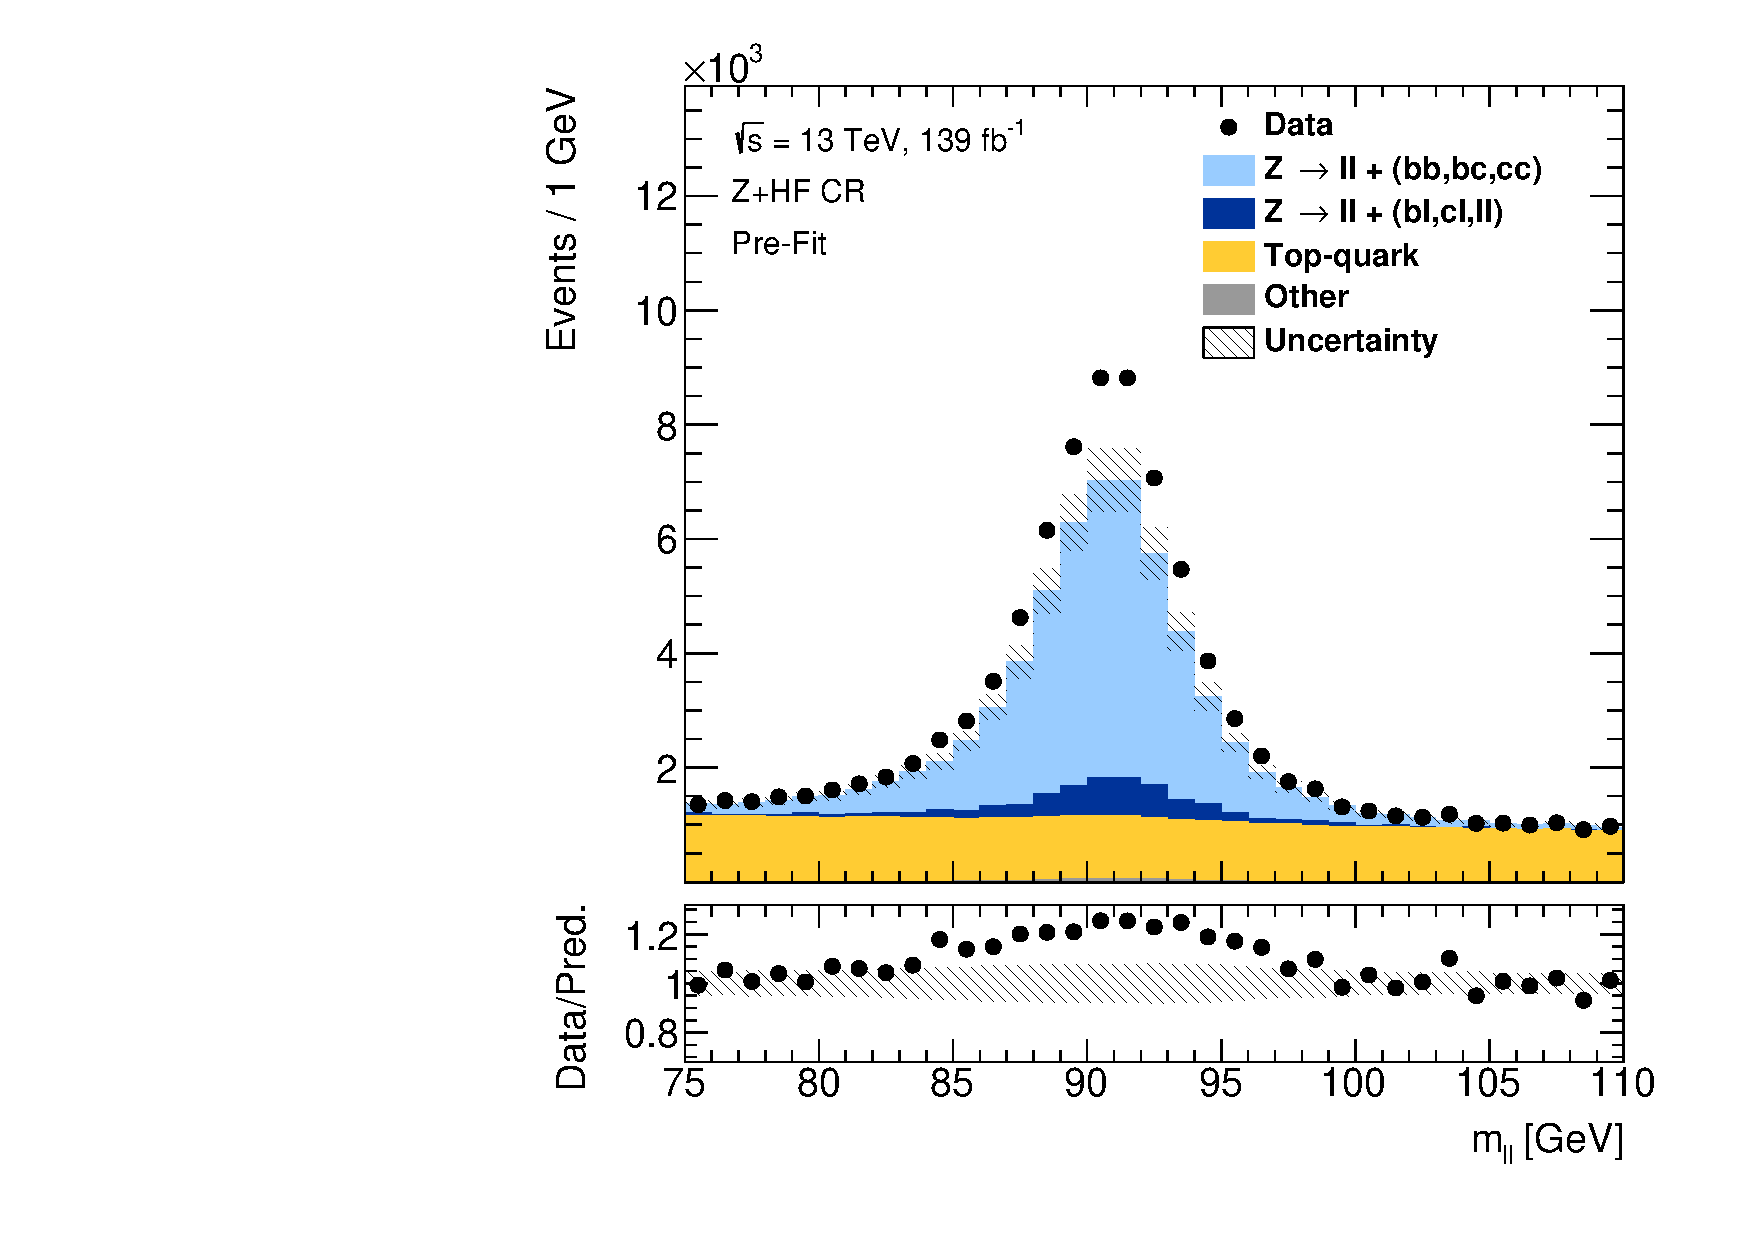
\includegraphics[width=\textwidth]{zhfcr/Region_BMin0_incJet1_Y2015_DZllbbCR_T2_L2_distmLL_J2_Prefit_fixed}
    \subcaption{Pre-fit}
    \label{fig:zcr_mll_prefit}
  \end{subfigure}\hfill%
  \begin{subfigure}{.485\textwidth}
    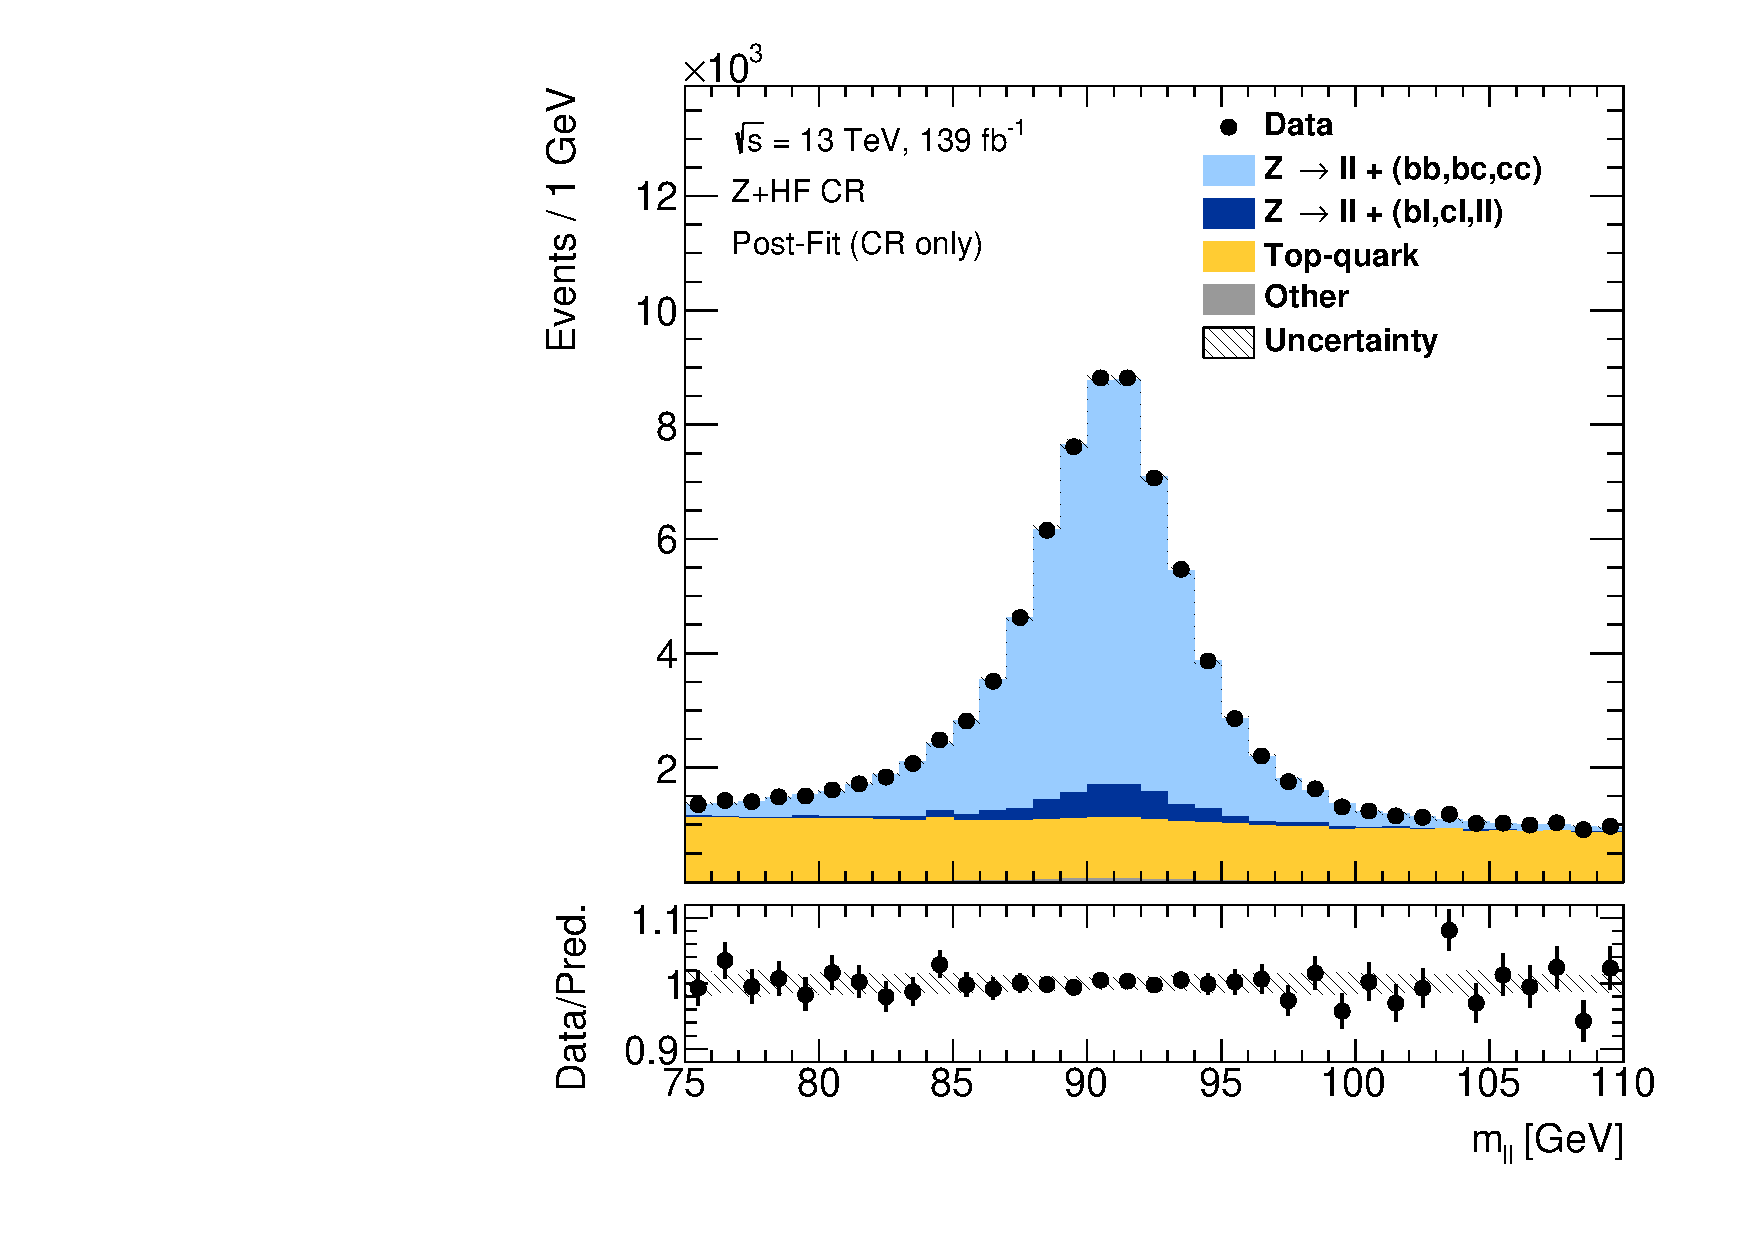
\includegraphics[width=\textwidth]{zhfcr/Region_BMin0_incJet1_Y2015_DZllbbCR_T2_L2_distmLL_J2_GlobalFit_conditionnal_mu0_fixed}
    \subcaption{Post-fit (\ZHF control region only)}
    \label{fig:zcr_mll_postfit}
  \end{subfigure}

  \caption{Distribution of the invariant di-lepton mass for the
    combination of electron- and muon-channel in the Z+HF control
    region before (a) and after (b) the likelihood fit restricted to
    the control region. The contribution of \Zjets is sub-divided into
    cases where both $b$-jet candidates are matched to heavy flavour
    quarks ($b$ or $c$) and cases where at most one candidate is
    matched to heavy flavour quarks at generator-level. Prior to the
    fit the \Zjets background is normalised to cross section
    predictions at NNLO~\cite{Anastasiou:2003ds}. All statistical and
    systematic uncertainties are included.}
\end{figure}

% ATLAS_norm_Zhf    1.3856e+00 +/-  1.19e-01
% ATLAS_norm_ttbar    9.7290e-01 +/-  3.92e-02
% Included in the SR fits: Systematic uncertainties are introduced at a later stage...
The \ZHF control region is included in simultaneous fits of signal and
control regions to provide constraints on the normalisation of the
\ZHF background. Details on systematic uncertainties and the fit model
are discussed
in~\Cref{sec:uncertainties,sec:statistical_analysis}. Restricting the
maximum likelihood fit to the control region yields estimates of the
normalisation factors of \num{1.39 \pm 0.12} and \num{0.97 \pm 0.04}
for \ZHF and \ttbar, respectively. The quoted normalisation factors
include all statistical and systematic
uncertainties. \Cref{tab:zcr_yields} and \Cref{fig:zcr_mll_postfit}
show the event yields and \mll distribution after the fit.



% When performing the likelihood fit in the control region only, the
% estimated normalisation factors are~\num{1.39 \pm 0.12} for the \ZHF
% and~\num{0.97 \pm 0.04} for the \ttbar background. The abundance of
% \ttbar events in the control region provides stringent constraints
% on the normalisation of the \ttbar background in addition to
% constraining the normalisation of the \ZHF background. The post-fit
% event yields and \mll distribution is shown in~\Cref{tab:zcr_yields}
% and~\Cref{fig:zcr_mll_postfit}, respectively.

%%% Local Variables:
%%% mode: latex
%%% TeX-master: "../../phd_thesis"
%%% End:
